
%%%%%%%%%%%%%%%%%%%%%%%%%%%%%%%%%%%%%%%%%
% Structured General Purpose Assignment
% LaTeX Template
%
% This template has been downloaded from:
% http://www.latextemplates.com
%
% Original author:
% Ted Pavlic (http://www.tedpavlic.com)
%
% Note:
% The \lipsum[#] commands throughout this template generate dummy text
% to fill the template out. These commands should all be removed when
% writing assignment content.
%
%%%%%%%%%%%%%%%%%%%%%%%%%%%%%%%%%%%%%%%%%

%	PACKAGES AND OTHER DOCUMENT CONFIGURATIONS

\documentclass[a4paper]{article}
\usepackage[utf8]{inputenc}
\usepackage[T1]{fontenc}
\usepackage[english]{babel}
\usepackage{fancyhdr} % Required for custom headers
\usepackage{lastpage} % Required to determine the last page for the footer
\usepackage{extramarks} % Required for headers and footers
\usepackage{graphicx} % Required to insert images
\usepackage{amsmath,amssymb,amsthm,amsfonts}
\usepackage{cleveref}

% Margins
\topmargin=-0.45in
\evensidemargin=0in
\oddsidemargin=0in
\textwidth=6.3in
\textheight=9.6in
\headsep=0.25in

\linespread{1.1} % Line spacing

% Set up the header and footer
\pagestyle{fancy}
\lhead{\hmwkAuthorName} % Top left header
\chead{\hmwkTitle} % Top center header
\rhead{\hmwkClass} % Top right header
\lfoot{} % Bottom left footer
\cfoot{} % Bottom center footer
\rfoot{Page\ \thepage\ of\ \pageref{LastPage}} % Bottom right footer

\renewcommand\headrulewidth{0.4pt} % Size of the header rule
\renewcommand\footrulewidth{0.4pt} % Size of the footer rule

\setlength\parindent{0pt} % Removes all indentation from paragraphs

\setcounter{secnumdepth}{0} % Removes default section numbers

%	NAME AND CLASS SECTION

\newcommand{\hmwkTitle}{Classical Loop-Shaping} % Assignment title
\newcommand{\hmwkClass}{EL2520} % Course/class
\newcommand{\hmwkClassName}{Control Theory and Practice} % Course/class
\newcommand{\hmwkAuthorName}{Isaksson, Oscarsson} % Your name

%	TITLE PAGE

\title{
	\vspace{1.5in}
	\textmd{\textbf{\hmwkClass\ -- \hmwkClassName}}\\
	\vspace{0.2in}
	\textmd{\textbf{\hmwkTitle}}\\
	\normalsize\vspace{0.1in}\small{\today}\\
	\vspace{2in}
}
\author{
	Martin Isaksson\\
	misakss@kth.se\\
	920622-3373
	\and
	Oscar Oscarsson\\
	y@kth.se\\
	YYMMDD-NNNN
}
\date{}

%%%%%%%%%%%%%%%%%%%%%%%%%%%%%%%%%%%%%%%%%%%%%%%%%%

\begin{document}

\maketitle

\vfill
\begin{abstract}
	In this report, we consider the classical loop-shaping procedure for control design \ldots
\end{abstract}

\newpage


%%%%%%%%%%%%%%%%%%%%%%%%%%%%%%%%%%%%%%%%%%%%%%%%%%

\section{Basics}
A system is modeled by the transfer function (given in \cite{exercise})
\begin{equation}
	G(s) = \frac{3(-s+1)}{(5s+1)(10s+1)}.
	\label{eq:system}
\end{equation}

We will design a lead-lag compensator $F$ such that the closed loop system in \cref{fig:block_diagram} fulfills the following specification:
\begin{itemize}\setlength{\itemsep}{-2pt}
	\item Crossover frequency $\omega_c = 0.4$ rad/s.
	\item Phase margin $\phi_m = 30^\circ$.
	\item No stationary error for a step response.
\end{itemize}

\begin{figure}[h!]
	\begin{center}
		\includegraphics[width=0.5\textwidth]{tex/figs/ext/loopshape_system}
	\end{center}
	\caption{Closed loop block diagram, where $F$--controller, $G$--system, $r$--reference signal, $u$--control signal, $d$--disturbance signal, $y$--output signal, $n$--measurement noise.}
	\label{fig:block_diagram}
\end{figure}

We follow the procedure from \cite{basic_book} to determine the parameters $K, \beta, \tau_D, \tau_i, \gamma$ in the lead-lag compensator
\begin{equation}
	F(s) = K \frac{\tau_D s + 1}{\beta \tau_D s + 1} \frac{\tau_I s + 1}{\tau_I s + \gamma}.
	\label{eq:lead_lag}
\end{equation}
The system's phase, $\arg(G(i\omega_c)) = -160^\circ$, is determined from the Bode diagram in \cref{fig:bode_diagram}.

\begin{figure}[h!]
	\begin{center}
		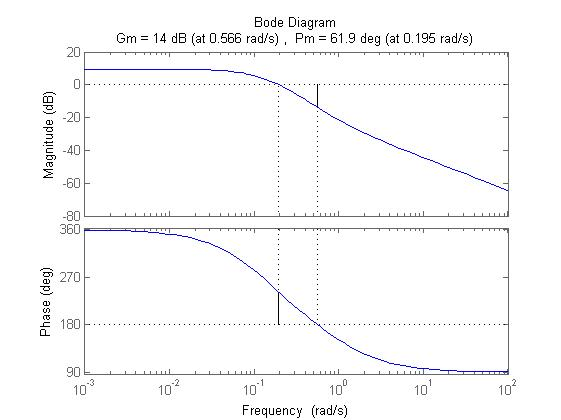
\includegraphics[width=0.7\textwidth]{G_margin}
	\end{center}
	\caption{Bode diagram for system $G(s)$ in \eqref{eq:system}.}
	\label{fig:bode_diagram}
\end{figure}

Thus, the necessary phase shift is
\[
	30^\circ - (-160^\circ - -180^\circ) + 8^\circ = 18^\circ,
\]
where an extra $8^\circ$ has been added to account for the lag-part. The first parameter can now be selected from \cite[fig. 5.13]{basic_book} as $\beta = 0.51$.

\ldots

The final controller is given by \cref{eq:lead_lag} with the parameters in \cref{tb:lead_lag_parameters}.
\begin{table}
\begin{center}
	\begin{tabular}{|c|c|c|c|c|}
		\hline
		$K$ & $\beta$ & $\tau_D$ & $\tau_i$ & $\gamma$\\
		\hline
		2.0377 & 0.51 & 3.5007 & 25 & 0\\
		\hline
	\end{tabular}
\end{center}
\caption{Parameters for the lead-lag compensator.}
\label{tb:lead_lag_parameters}
\end{table}

\ldots

The rise time and overshoot is determined form the step response in \cref{fig:step_response}, and given in \cref{tb:response}.

\begin{figure}[h!]
	\begin{center}
		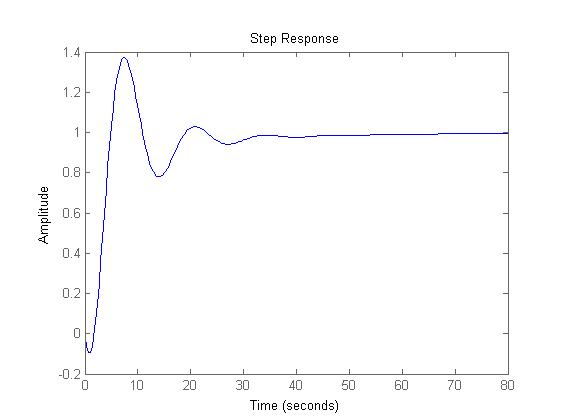
\includegraphics[width=0.7\textwidth]{Step_Gc_1}
	\end{center}
	\caption{Step response for the closed loop system in \cref{fig:block_diagram}, with the lead-lag compensator.}
	\label{fig:step_response}
\end{figure}

\begin{table}[h!]
\begin{center}
	\begin{tabular}{|c|c|c|c|}
		\hline
		$\omega_B$ [rad/s] & $M_T$ [dB] & $T_r$ [s] & $M$ [\%] \\
		\hline
		0.7811 & 5.8771 & 2.3921 & 37.1793\\
		\hline
	\end{tabular}
\end{center}
\caption{Closed loop system characteristics.}
\label{tb:response}
\end{table}

\begin{table}[h!]
\begin{center}
	\begin{tabular}{|c|c|c|c|c|}
		\hline
		$K$ & $\beta$ & $\tau_D$ & $\tau_i$ & $\gamma$\\
		\hline
		1.3684 & 0.23 & 5.2129 & 25 & 0\\
		\hline
	\end{tabular}
\end{center}
\caption{Parameters for the lead-lag compensator.}
\label{tb:lead_lag_parameters}
\end{table}

\begin{figure}[h!]
	\begin{center}
		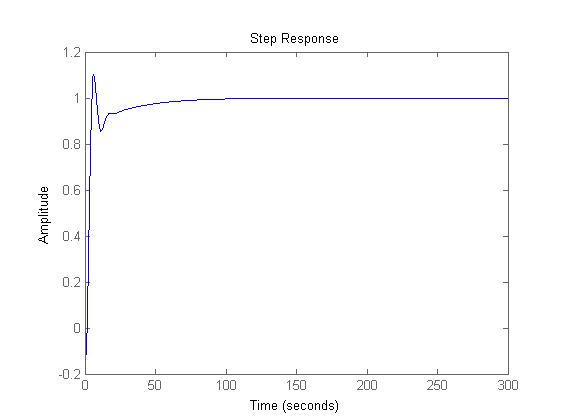
\includegraphics[width=0.7\textwidth]{Step_Gc_2}
	\end{center}
	\caption{Step response for the closed loop system in \cref{fig:block_diagram}, with the lead-lag compensator.}
	\label{fig:step_response}
\end{figure}

\begin{table}[h!]
\begin{center}
	\begin{tabular}{|c|c|c|c|}
		\hline
		$\omega_B$ [rad/s] & $M_T$ [dB] & $T_r$ [s] & $M$ [\%] \\
		\hline
		0.9341 & 1.1032 & 2.4054 & 10.3174\\
		\hline
	\end{tabular}
\end{center}
\caption{Closed loop system characteristics.}
\label{tb:response}
\end{table}

\ldots

\section{Disturbance attenuation}
\ldots

\section{Conclusions}
\ldots

\begin{thebibliography}{9}

\bibitem{exercise}
EL2520 Control Theory and Practice Advanced Course, \emph{Computer Exercise: Classical Loop-Shaping}, 2014.

\bibitem{basic_book}
T. Glad and L. Ljung, \emph{Reglerteknik, Grundläggande teori}, Studentlitteratur, 2006.

\end{thebibliography}


%%%%%%%%%%%%%%%%%%%%%%%%%%%%%%%%%%%%%%%%%%%%%%%%%%

\newpage
\section{Some reminders}
\begin{itemize}
	\item Write clear and concise, but comprehensible. No novels!
	\item The report should be self-contained, don't assume the reader knows the lab instructions.
	\item However, don't repeat material from the course book, instead, use references.
	\item Make sure that all results and figures are reproducible.
	\item Start with a \emph{short} summary of the results and the contents of the report.
	\item Motivate all the choices you have done.
	\item Show results in tables and figures that are easy to compare.
	\item Introduce figures in the text where it is needed, and remember to describe what the figure shows, what the axes corresponds to and what the results are.
	\item Be specific in your writing, and avoid vague expressions such as ``some'' and ``not so good''.
	\item Check grammar your and speling.
\end{itemize}

\end{document}
